\documentclass[letter,12pt]{article}
\usepackage[letterpaper,right=1in,left=1in,top=1in,bottom=1in]{geometry}
\usepackage{setspace}

\usepackage[utf8]{inputenc}   % allows input of special characters from keyboard (input encoding)
\usepackage[T1]{fontenc}      % what fonts to use when printing characters       (output encoding)
\usepackage{amsmath}          % facilitates writing math formulas and improves the typographical quality of their output
\usepackage[hyphens]{url}     % adds line breaks to long urls
\usepackage[pdftex]{graphicx} % enhanced support for graphics
\usepackage{tikz}             % Easier syntax to draw pgf files (invokes pgf automatically)
\usetikzlibrary{arrows}

\usepackage{mathptmx}           % set font type to Times
\usepackage[scaled=.90]{helvet} % set font type to Times (Helvetica for some special characters)
\usepackage{courier}            % set font type to Times (Courier for other special characters)

\usepackage[longnamesfirst, sort]{natbib}\bibpunct[]{(}{)}{,}{a}{}{;} % handles biblio and references 

\usepackage{rotating}         % sideway tables and figures that take a full page
\usepackage{caption}          % allows multipage figures and tables with same caption (\ContinuedFloat)

\usepackage{dcolumn}          % needed for apsrtable and stargazer tables from R to compile
\usepackage{arydshln}         % dashed lines in tables (hdashline, cdashline{3-4}, 
                              %see http://tex.stackexchange.com/questions/20140/can-a-table-include-a-horizontal-dashed-line)
                              % must be loaded AFTER dcolumn, 
                              %see http://tex.stackexchange.com/questions/12672/which-tabular-packages-do-which-tasks-and-which-packages-conflict


\newcommand{\mc}{\multicolumn}

%% TO ADD NOTES IN TEXT, PUT % BEFORE THE ONE YOU WANT DISABLED
%\usepackage[disable]{todonotes}                            % no show
\usepackage[colorinlistoftodos, textsize=small]{todonotes} % show notes
\newcommand{\emm}[1]{\todo[color=red!15, inline]{\textbf{Eric:} #1}}
\newcommand{\vp}[1]{\todo[color=green!15, inline]{\textbf{Vale:} #1}}
\newcommand{\ges}[1]{\todo[color=blue!15, inline]{\textbf{Ges:} #1}}

\usepackage{xr} % allows cross-ref to other file
\externaldocument{urge14}

\usepackage{tabularx}  % tabular with 1 column taking rest of \textwidth
\usepackage{longtable} % tables across multiple pages



\begin{document}

\title{On-line appendix for ``Presidents on the Fast Track: Fighting Floor Amendments with Restrictive Rules''}
\author{Eric Magar \\ ITAM \and
        Valeria Palanza \\ Univ.\ Católica de Chile \and  
        Gisela Sin \\ University of Illinois
}
\date{\today}
\maketitle

%\begin{center} \textbf{$\rightarrow$~~Preliminary draft~~$\leftarrow$} \\ (please inquire for new version, \small{\url{emagar@itam.mx}})  \end{center}

%% \begin{abstract}
%% \noindent Includes x, y, and z info
%% \end{abstract}

\tableofcontents

\doublespacing

\renewcommand\thefigure{A.\arabic{figure}} 
\renewcommand\thetable{A.\arabic{table}} 


%% %%%%%%%%%%%%%%%%%%%%%%%%
%% % APPENDIX STARTS HERE %
%% %%%%%%%%%%%%%%%%%%%%%%%%

\section{Chilean urgency types}

Congressional practice is well summarized by the library of Congress at \url{http://www.bcn.cl/ecivica/formacion/}. The congressional organic law (\emph{Ley Orgánica del Congreso}, arts.\ 26 and 27) gives presidents the following choices to qualify urgent bills:

\begin{enumerate}
\item Simple (\emph{urgencia simple}), providing Congress with 30 calendar days for bill consideration;
\item Supreme (\emph{urgencia suma}), providing 15 calendar days for consideration); and
\item Immediate discussion (\emph{discusión inmediata}), providing 6 calendar days.
\end{enumerate}

\noindent By defining what amounts to `simple urgency' only, the constitution sets a floor for the authority. Higher degrees of urgency included in the organic law are vulnerable to congressional majorities, which might be inclined to relax the deadlines available if it were in their interest. In fact, congress altered these deadlines once, in 2010: the organic law was amended in July of 2010, four months into the newly elected legislature (during Piñera's first administration), substantially relaxing the deadlines for the `immediate discussion' and `supreme urgency' types, originally set at 10 and 3 days, to 15 and 6 days respectively (our analysis controls for this change). `Simple urgency', with a 30 day deadline, remained unchanged. The urgency deadline applies to the receiving chamber only, not to the other chamber, but does apply to the conference committee should one be originated after both chambers have arrived at decisions. Also, urgency messages expire at the end of the ordinary period on March 10th every year, and the president may remove urgency at will, with immediate effects. 
To say more on the requirements to alter the established deadlines for each urgency type, we note that the Constitution (art.~66) sets a high bar for altering urgency deadlines by requiring the vote of four-sevenths ($\approx 57$ percent) of each chamber's membership for the passage and amendment of constitutional organic laws. While this qualified requirement is below the two-thirds needed for constitutional reform, no coalition has exceeded the organic law threshold in both chambers since the return to democracy. 

It is important to distinguish urgencies by type/degree because the \emph{Reglamento de la Cámara de Diputados} in the period mandated that supreme urgency qualification triggered restrictive floor consideration rules, whereas the highest and lowest urgency degrees did not. (In 2014 an amendment to the Rules expanded closed rules to two types of urgencies, but this falls outside the time span of our analysis.) For this reason, and unless otherwise noted, by urgency in Chile the article means `supreme urgency' qualifications only. 

% numbers produced in chillBill.r (above xtable command). Verify if changes have occurred since...
\begin{table}
\centering
\caption{Urgency type breakdown 1998--2014 (complement to Table \ref{T:billDescriptives})}\label{T:billDescriptivesPartB}
\begin{tabular}{llr}
    & Bills declared urgent                        &  frequency   \\ \hline
V   & Immediate discussion (once at least)         &         255  \\
    & as \% of introduced                          &   \emph{17}  \\ \hdashline
VI  & \textbf{Supreme urgency} (once at least)     &         540  \\
    & as \% of introduced                          &   \emph{37}  \\ \hdashline
VII & Simple urgency (once at least)               &         424  \\
    & as \% of introduced                          &   \emph{29}  \\ \hdashline
VIII& Any urgency (once at least)$^\dagger$          &         835  \\
    & as \% of declared urgent                     &   \emph{57}  \\
\hline
\multicolumn{3}{r}{\footnotesize{$^\dagger$ Categories V, VI, and VII not mutually-exclusive (see footnote \ref{fnNonExclusive}).}} \\
\end{tabular}
\end{table}

Table \ref{T:billDescriptivesPartB} reports urgency frequencies by degree type. Bills in the fast-track (panel VI) were more frequent than bills qualified at least once for either immediate discussion (17 percent) or simple urgency (29 percent).\footnote{\label{fnNonExclusive}We say once at least because bills can be qualified urgent more than once. This does not refer to the possibility that a bill is qualified urgent during lower chamber consideration, then again during Senate consideration (analysis, in fact, ignores all Upper Chamber urgency qualifications); but to the fact that, during Cámara consideration, one same bill often received many urgency designations---e.g., an initial simple urgency deadline is reset before its expiration, or replaced by supreme urgency. The modal urgent bill in the period received several such qualifications, sometimes renewing an urgency that was previously withdrawn. Other times the deadline for consideration was reset before the original expired, often more than once. Less common were cases changing one deadline by a shorter one. We plan to investigate the puzzling patterns of urgency chains in a separate project. Urgency chains imply that the absolute frequencies by types do not add up to the total in panel VIII.} Analysis ignores all `immedite discussion' and `simple urgency' qualifications (i.e., only panel VI is fast-track qualification). 

\section{Supreme urgency and the closed rule}

In the period we examine, the Cámara's standing rules explicitly precluded the second committee report for bills qualified with supreme urgency (\emph{urgencia suma}), ruling out the bill's second reading by mandating that general (i.e., first reading) and particular (i.e., second reading) considerations take place simultaneously. In other words, supreme urgency mandated a closed floor consideration rule, whereas other urgency types did not.

The text of the relevant Reglamento articles follows. Excerpts are from the standing rules adopted in March 10, 2002 (with text updated to March 2010).  

%%%%%%%%%%%%%%%%%%%%%%%%%%%%%%%
%% ReglamDip arts 188 y 189: %%
%%%%%%%%%%%%%%%%%%%%%%%%%%%%%%%
%% Art. 188. Cuando un proyecto sea declarado de "suma urgencia", se procederá a su discusión en la siguiente forma: No habrá segundo informe de Comisión y el proyecto deberá ser despachado por la Cámara en diez días, que se distribuirán así:
%% 1° Cinco días para el informe de Comisión.
%% 2° Tres días para el informe de la Comisión de Hacienda, si procediere.
%% 3° Dos días para la discusión y votación en la Sala.
%% La discusión se hará en general y particular a la vez. Sólo se admitirán a discusión y votación las indicaciones o disposiciones que, rechazadas por la Comisiones informantes, sean renovadas con las firmas de treinta Diputados que incluyan, a lo menos, a tres Jefes de Comités. Para tal efecto, los informes consignarán expresamente estas circunstancias.
%% Lo dispuesto en este número se debe entender sin perjuicio de lo establecido en el inciso segundo del artículo 132 (declaratoria de terminada la discusión).
%% ...
%% Art. 189. Cuando un proyecto sea declarado de "discusión inmediata", se procederá a su discusión y votación en la forma siguiente:
%% El proyecto deberá ser despachado por la Cámara en tres días, que se distribuirán así:
%% 1$^o$ Un día para el informe de la Comisión competente, que puede ser verbal o escrito.
%% 2$^o$ Un día para el informe de la Comisión de Hacienda, si procediere, que puede ser verbal o escrito.
%% 3$^o$ Un día para la discusión y votación del proyecto.
%% Lo dispuesto en este N$^o$ 3 deberá entenderse sin perjuicio de lo establecido en el inciso segundo del artículo 132 (renuncia de Comités a su tiempo).
%% Para los demás trámites Constitucionales tendrá la Cámara un día adicional.
%% La discusión de estos proyectos se hará en general y particular a la vez. No serán sometidos a segundo informe.
%% La Ley Orgánica no menciona nada acerca de restrictive rules.

\singlespacing

Art.~188. When a project is qualified as ``\textbf{supreme urgency}'', its discussion shall proceed thus: \textbf{There will be no second committee report} and the project shall be dispatched by the Chamber in ten days [...] \textbf{Discussion shall be general and particular at once}. Only amendments and additions rejected in committee, but renewed with the signature of thirty Deputies, including at least three committee chairs, shall be admitted for discussion and vote [...]

(In Spanish: Art.~188. \emph{Cuando un proyecto sea declarado de ``\textbf{suma urgencia}'', se procederá a su discusión en la siguiente forma: \textbf{No habrá segundo informe de Comisión} y el proyecto deberá ser despachado por la Cámara en diez días [...]
\textbf{La discusión se hará en general y particular a la vez}. Sólo se admitirán a discusión y votación las indicaciones o disposiciones que, rechazadas por la Comisiones informantes, sean renovadas con las firmas de treinta Diputados que incluyan, a lo menos, a tres Jefes de Comités [...]})

\bigskip

Art.~189. When a project is qualified as ``\textbf{immediate discussion}'', its discussion shall proceed thus: The project shall be dispatched by the Chamber in three days [...]
\textbf{Discussion of these projects shall be general and particular at once. They will not be subject to a second committee report.}

(In Spanish: Art.~189. \emph{Cuando un proyecto sea declarado de ``\textbf{discusión inmediata}'', se procederá a su discusión y votación en la forma siguiente:
El proyecto deberá ser despachado por la Cámara en tres días [...]
\textbf{La discusión de estos proyectos se hará en general y particular a la vez. No serán sometidos a segundo informe.}})

\doublespacing

Cámara rules were amended in 2014 to generalize closed consideration rules for urgencies regardless of degree. This, however, falls outside the time span of the data we analyze.


\section{Variable definitions and descriptive statistics}

Unless otherwise noted, data are from the Cámara's web page at \url{https://www.camara.cl/}.

\subsection{Dichotomous variables}\label{s:descriptives-dummies}

\begin{footnotesize}
\singlespacing
\begin{tabularx}{\textwidth}{lXrrr} % X type column fills rest of space
 Variable                      & Definition &   $=0$ &  $=1$ & Total \\ [.5ex] \hline
\emph{Fast-tracked Bill} (Dep.~Var.) & Equal 1 for bills qualified as supreme urgent (\emph{urgencia suma}) once or more in the Cámara, equal 0 otherwise.          &    927  &   540 & 1,467 \\ [.5ex] %[-.25ex]
%                         &        &   .632 &  .368 &   1 \\ [.5ex]
\\ [-1ex]
\\ [-1ex]
\emph{Co-partisan Comm.~Chair}       & Equal 1 for bills referred to any Cámara committee whose chair belongs in the president's party, equal 0 otherwise.          &    832 &   635 & 1,467 \\ [.5ex] %[-.25ex]
%                                     &        &   .567 &  .433 &   1   \\ [.5ex]
\\ [-1ex]
\emph{Coalition Comm.~Chair}         & Equal 1 for bills referred to any Cámara committee whose chair belongs in the president's electoral list, equal 0 otherwise. &     99 & 1,368 & 1,467 \\ [.5ex] %[-.25ex]
%                                     &        &   .067 &  .933 &   1   \\ [.5ex]
\\ [-1ex]
\emph{Multiple Referrals}            & Excluding the Cámara's Hacienda committee, equal 1 for bills referred to more than one of the Cámara's standing committee (or a joint committee), equal 0 otherwise. &  1,096 &   371 & 1,467 \\ [.5ex] %[-.25ex]
%                                     &        &   .747 &  .253 &   1   \\ [.5ex]
\\ [-1ex]
\emph{Hacienda Referral}             & Equal 1 for bills referred to the Cámara's Hacienda (finance) committee, equal 0 otherwise.                                  &    732 &   735 & 1,467 \\ [.5ex] %[-.25ex]
%                                     &        &   .499 &  .501 &   1   \\ [.5ex]
\\ [-1ex]
\emph{Introduced in Senate}          & Equal 1 for bills originally introduced and passed in the upper chamber of Congress, equal 0 otherwise.                      &  1,224 &   243 & 1,467 \\ [.5ex] %[-.25ex]
%                                     &        &   .834 &  .166 &   1   \\ [.5ex]
\\ [-1ex]
\emph{Senate Majority}               & Equal 1 for bills introduced during a period when the president's electoral list controlled half or more of seats in the upper chamber of Congress, equal 0 otherwise. &    512 &   955 & 1,467 \\ [.5ex] %[-.25ex]
%                                     &        &   .349 &  .651 &   1   \\ [.5ex]
\\ [-1ex]
\emph{Relax Deadlines}               & Equal 1 for bills introduced on or after July 11th, 2010, when a reform to the Ley Orgánica del Congreso relaxing deadlines for consideration of supreme urgent bills went into effect, equal 0 otherwise. &  1,094 &   373 & 1,467 \\ [.5ex] %[-.25ex]
%                                     &        &   .746 &  .254 &   1   \\ [.5ex]
\\ [-1ex]
\emph{1998--2002}                    & Equal 1 for bills introduced between Mar.\ 1st, 1998 and Feb.\ 28th, 2002 inclusive, equal 0 otherwise. &  1,195 &   272 & 1,467 \\ [.5ex] %[-.25ex]
%                                     &        &   .815 &  .185 &   1   \\ [.5ex]
\\ [-1ex]
\emph{2002--2006}                    & Equal 1 for bills introduced between Mar.\ 1st, 2002 and Feb.\ 28th, 2006 inclusive, equal 0 otherwise.       &  1,067 &   400 & 1,467 \\ [.5ex] %[-.25ex]
%                                     &        &   .727 &  .273 &   1   \\ [.5ex]
\\ [-1ex]
\emph{2006--2010}                    & Equal 1 for bills introduced between Mar.\ 1st, 2006 and Feb.\ 28th, 2010 inclusive, equal 0 otherwise.       &  1,075 &   392 & 1,467 \\ [.5ex] %[-.25ex]
%                                     &        &   .733 &  .267 &   1   \\ [.5ex]
\\ [-1ex]
\emph{2010--2014}                    & Equal 1 for bills introduced between Mar.\ 1st, 2010 and Feb.\ 28th, 2014 inclusive, equal 0 otherwise.       &  1,064 &   403 & 1,467 \\ [.5ex] %[-.25ex]
%                                     &        &   .725 &  .275 &   1   \\
\hline
\end{tabularx}
\doublespacing
\end{footnotesize}
  
\subsection{Continuous variables}

There are two continuous variables in the equation. As reported in the text, both were normalized in order to accelerate convergence of the mixed effects estimation (Model 4). We used the normalized versions in models 1--3 to render coefficients comparable. Descriptive statistics below correspond to the un-normalized values.

\begin{footnotesize}
\singlespacing
\begin{tabularx}{\textwidth}{lXrrrrrrr} % X type column fills rest of space
          Variable  & Definition &  Min.&  Q1 & Med. & Mean &  Q3  &  Max. &   sd \\ [.5ex] \hline
\emph{Year Remaining}& Equal $d*100/365$, where $d$ is obtained thus: counting the first day of the legislative year (Mar.\ 1st) as day 365 and the last day of the legislative year (Feb. 28th) as day 1, $d$ corresponds to the bill initiation's day.     &  0   &  27 & 51   & 51.5 & 75   & 100   &   27.1 \\ [.5ex]
\\ [-1ex]
\emph{Pres.~Approval}& Percent approving minus percent disapporving of the president's job. Data are from the Centro de Estudios Públicos' bi-yearly face-to-face opinion polls, available at \url{www.cepchile.cl}. &-39.2 & -8 &  10.7 &  9.5 & 22.3 &  66.3 &   24.2 \\ \hline
\end{tabularx}
\doublespacing
\end{footnotesize}
  
  \section{Temporal dimension}\label{s:temp-dim}

Our empirical investigation deals with a theoretically interesting and substantively important aspect of the urgency authority in Chile. But legislative histories contain a wealth of information we do not analyze. We summarize patterns in urgency incidence that inform methodological choices that we made. In particular, the descriptive exercise highlights the temporal dimension of urgency authority that led us to control the legislative calendar in the estimation. 

The executive indicates a bill's urgent status, or makes modifications to such status, through messages (\emph{mensajes}) to the relevant chamber of Congress. An \emph{original urgency} is a message compelling action on legislation with non-urgent status in the chamber. \emph{Non-original} messages extend, modify, or withdraw the bill's urgent status. The manuscript analyzes any message, original or not, issuing supreme urgency. Since we code this with a dummy,

As defined in section \ref{s:descriptives-dummies}, the manuscript's dependent variable equals 1 for bills with any message, original or not, issuing supreme urgency, 0 otherwise. The dichotomous nature of the variable, however, makes this it equivalent to original supreme urgency messages, as subsequent supreme urgency qualifications do not increase the value beyond 1. 

% latex table generated in R 3.1.2 by xtable 1.7-4 package
% Wed Feb  4 17:24:48 2015
\begin{table}
\centering
\begin{tabular}{rrrrr|r}
      & 1998--2002 & 2002--06 & 2006--10 & 2010--14 & 1998--2014 \\ \hline
 \multicolumn{5}{c|}{\textbf{Part A. Individual messages}} \\
 Immediate discussion& 5  & 5  & 3  & 3  & 3 \\ 
 supreme             & 14 & 13 & 9  & 12 & 11 \\ 
 simple              & 24 & 18 & 13 & 6  & 12 \\ \hdashline
 Shorten deadline    & 2  & 3  & 2  & 5  &  4 \\ 
 Extend deadline     & 39 & 42 & 43 & 60 & 49 \\ \hdashline
 Withdraw (immediate)& 1  & 2  & 2  & 2  &  2 \\ 
 Withdraw (supreme)  & 6  & 9  & 13 & 8  & 10 \\ 
 Withdraw (simple)   & 8  & 9  & 16 & 3  & 9  \\ \hline
 Total messages      & 100 & 100 & 100 & 100 & 100 \\ 
(N)                  & (1,218) & (1,821) & (4,908) & (5,611) & (13,558)\\ 
\\ [-1.5ex]
 \multicolumn{5}{c|}{\textbf{Part B. Urgency chains}}  \\
Immediate, singleton        & 8  & 8  & 4  & 5  &   5  \\
Immediate, extend           & 4  & 3  & 3  & 4  &   3  \\
Immediate, withdraw         & 1  & 1  & 1  & 2  &   1  \\
Immediate, extend, withdraw & 2  & 4  & 4  & 3  &   3  \\ \hdashline
Supreme, singleton          & 12 & 8  & 4  & 8  &   7  \\
Supreme, extend             & 9  & 9  & 4  & 17 &  10  \\
Supreme, withdraw           & 4  & 2  & 2  & 4  &   3  \\
Supreme, extend, withdraw   & 11 & 17 & 26 & 27 &  23  \\ \hdashline
Simple, singleton           & 11 & 5  & 3  & 3  &   4  \\
Simple, extend              & 18 & 17 & 3  & 10 &  10  \\
Simple, withdraw            & 2  & 3  & 2  & 2  &   2  \\
Simple, extend, withdraw    & 19 & 23 & 44 & 14 &  26  \\ \hline
Total chains                & 100 & 100 & 100 & 100 & 100  \\
(N)                         & (369) & (609) & (1,160) & (1,204) &(3,342) \\ 
Messages in mean chain      & 3.3   & 3.0   & 4.2     & 4.7     & 4.1 \\ \hline
% Senate status       & \emph{tied} & \emph{tied} & \emph{gov.} & \emph{opp.} & \\
\end{tabular}
\caption{Urgency messages and urgency chains. Chains (212 in total) initiated in the period but targeting bills proposed before the period are not considered.}\label{t:freqUrg}
\end{table}

Table \ref{t:freqUrg} inspects urgency messages and offers a finer-grained perspective. The sheer number of messages is appalling: 13,558 in the 16-year period, reaching averages of 71 monthly messages and 10 messages for every bill declared urgent in the period. Message frequency rose substantially from every four-year Legislature reported to the next. President Bachelet (2006--10) was responsible for the steepest hike in urgency incidence, issuing almost three times more messages relative to the previous Legislature and pushing the monthly average above 100. 

Also noteworthy is that just 26 percent of messages in the full period were original urgencies. Among original urgency messages, `act now' notice frequency (3 percent of messages) was one-fourth the frequency of `two week' and `one month' notices (11 and 12 percent, respectively). The literature has overlooked non-original urgency, which amounted to nearly three out of four messages in the period. Modifications included deadline changes and the withdrawal of the bill's urgent status altogether. Deadline changes mostly involved an extension of the period for bill consideration. Accounting for nearly half of all messages, deadline extensions were the modal message in every Legislature considered. Those cutting deadlines short were much rarer, 4 percent of all. And, with variance across Legislatures, urgency withdrawals were common too, two-fifths overall and nearly one-third in 2006--10. Urgency withdrawal is puzzling and suggests further dimensions of bargaining with the urgency authority not addressed here, but worth keeping in mind. 

So many non-original messages imply that urgency chains are common.\footnote{Formally, deadline changes consist of two paired messages in the source: one withdrawing the original urgency, another setting the new deadline. Paired withdrawal messages are excluded from the numbers reported, so as to retain only withdrawals actually terminating a bill's urgent status.} An \emph{urgency chain} is a series of chronologically connected urgency messages on the same piece of legislation, non-original messages adding links by modifying the urgency before the original deadline expires. Declaring legislation urgent is typically not a single shot affair. One example is legislation making split-couple parents equally responsible in rearing their children. The bill received a one month notice on 22 June 2011 (bolet\'in 7007--18). As the deadline neared, the C\'amara's Constitution, Law, and Justice committee requested more time to merge the proposal with two others; on 2 August, the deadline was duly pushed four weeks ahead. (we coded deadlines using business days, so the expiration was still ahead despite more than 30 calendar days had gone by.) Five other similar messages were issued, weaving a seven-link chain with a final deadline in March 2012.\footnote{Messages in the primary source were coded as extra chain links whenever issued on or before a bill's urgency deadline and sent to the same chamber. In most cases, the new message was paired to a withdrawal message, easing chain identification. For (relatively few) cases not reporting the paired withdrawal message's date, using calendar instead of business days might reclassify some messages out of chains.} As the Table's bottom reports, the average chain had 4.1 links (the longest reached 71). 

% \begin{table}
% \begin{center}
% \begin{tabular}{rrr}
% Number of &      Bill &     \\
% messages  & frequency &  ~~~~~~~~\% \\ \hline
% %None              &  5635     &     \\
% 1                 &  214      &  \emph{16}   \\
% 2                 &  242      &  \emph{18}   \\
% 3                 &  145      &  \emph{11}   \\
% 4                 &  115      &  \emph{8}    \\
% 5                 &  104      &  \emph{8}    \\
% 6-10              &  236      &  \emph{17}   \\
% 11-20             &  183      &  \emph{13}   \\
% 21-40             &  99       &  \emph{7}    \\
% 41-71             &  24       &  \emph{2}    \\
% Total             & 1,362     & \emph{100}   \\ \hline
% \end{tabular}
% \caption{Urgent bills classified by number of urgency messages received}\label{T:billFreqByNurg}
% \end{center}
% \end{table}

% Other interesting patterns in urgency authority usage are discernible in bill histories. Assessing how large the subset of bills receiving one or more urgency messages is conveys a minimalist perspective of the urgency authority. As shown in table \ref{T:billFreqByNurg}, most bills in this subset (84 percent) in fact received many such messages, and a substantial portion (40 percent) received between 6 and 71 urgency messages. This raises another puzzle for research. Are presidents reiterating urgency messages because of Congressional inaction? Extending the deadline may help the president save face when legislative non-compliance is imminent. Or are presidents micro-managing select-bill consideration in committee, monitoring a report's progress and then sending recommendations in the message extending the deadline? The source indicates the arrival of presidential messages but does not include their actual contents, nor those of committee reports. Archival research to retrieve those documents would do wonders in answering these questions. 

%A bicameral process operating on a single-round navette \citep{tsebelis.money.1997}---bills migrate from originating to revising chamber, back to originating if amended, and finally to conference if inter-cameral differences persist---offers, at most, four clear instances for repeated urgency authority use. Yet, as table \ref{T:billFreqByNurg} reports, nearly half of urgent bills (47 percent) received five messages or more. A handful of bills received several dozen messages! 

\begin{figure}
\begin{center}
 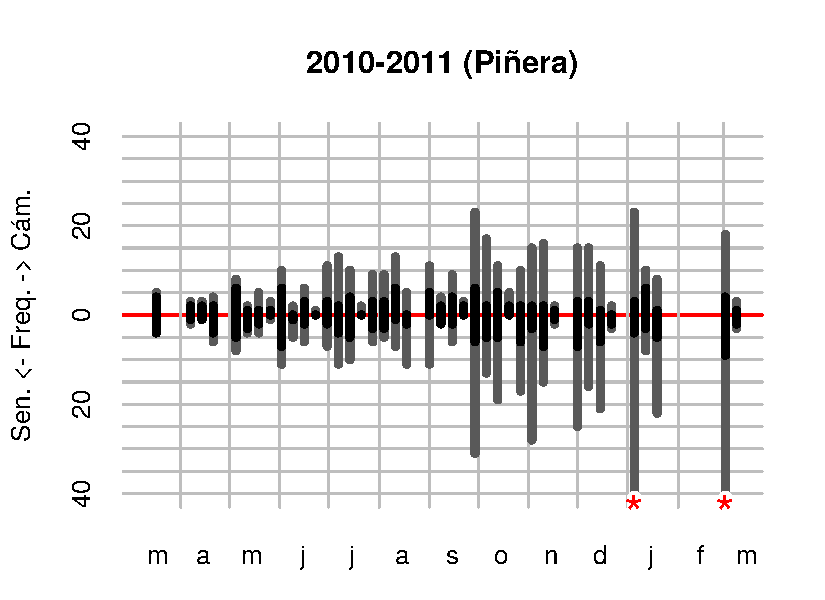
\includegraphics[width=.65\columnwidth]{../graphs/urgenciasHistog2010.pdf}
\begin{tabular}{cccc}
    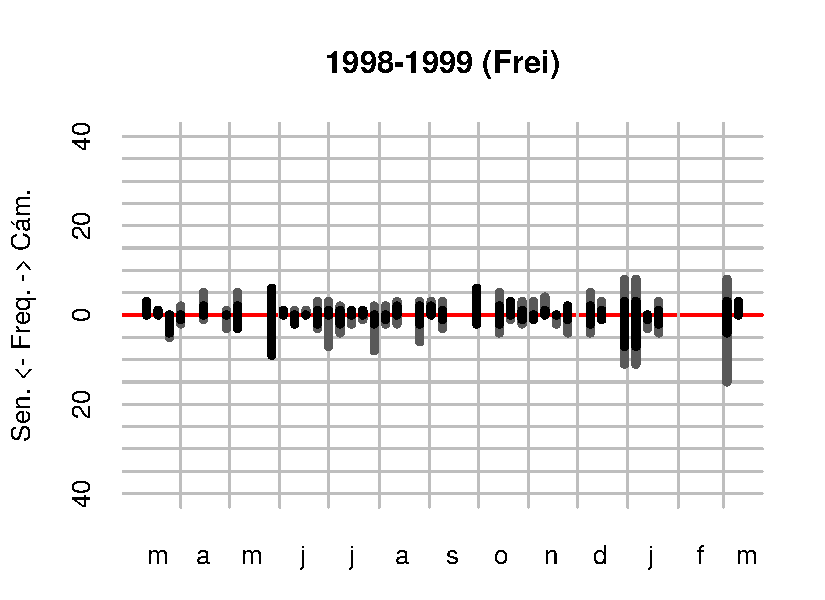
\includegraphics[width=.22\columnwidth]{../graphs/urgenciasHistog1998.pdf} &
    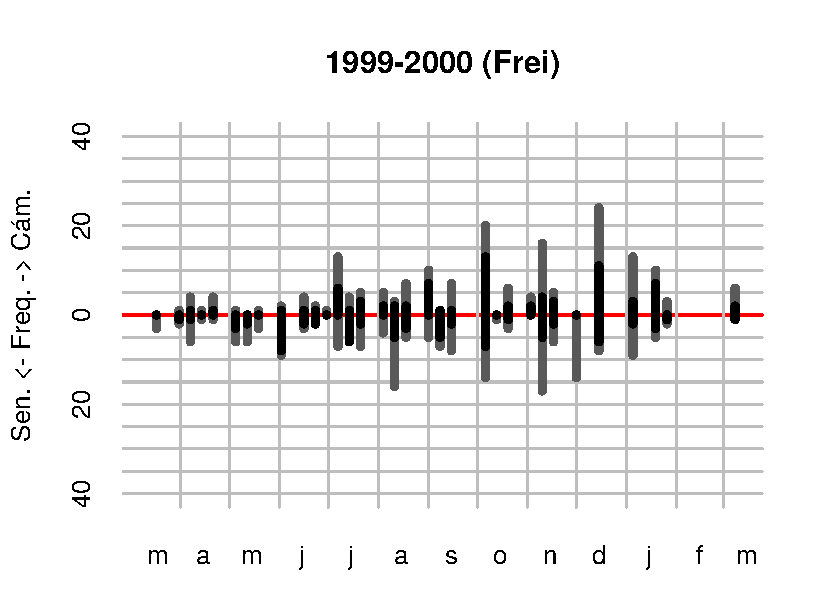
\includegraphics[width=.22\columnwidth]{../graphs/urgenciasHistog1999.pdf} &
    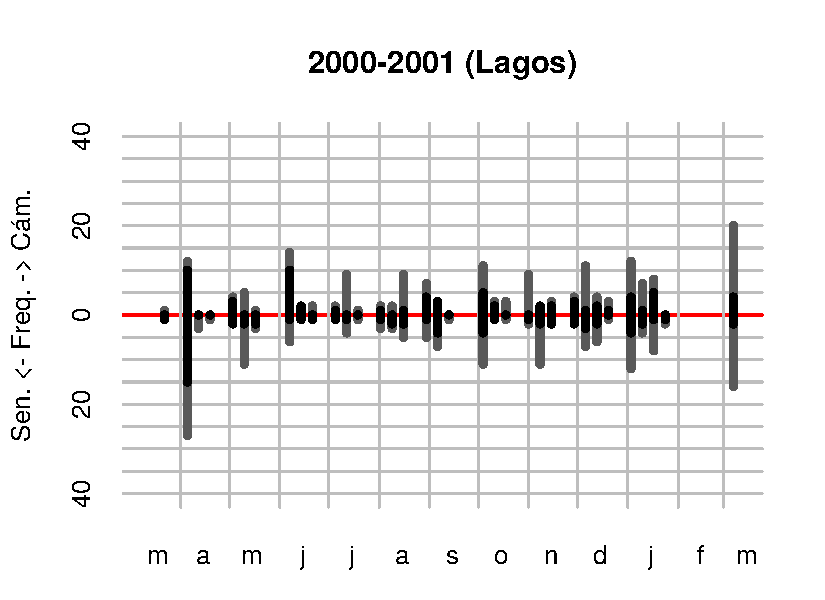
\includegraphics[width=.22\columnwidth]{../graphs/urgenciasHistog2000.pdf} &
    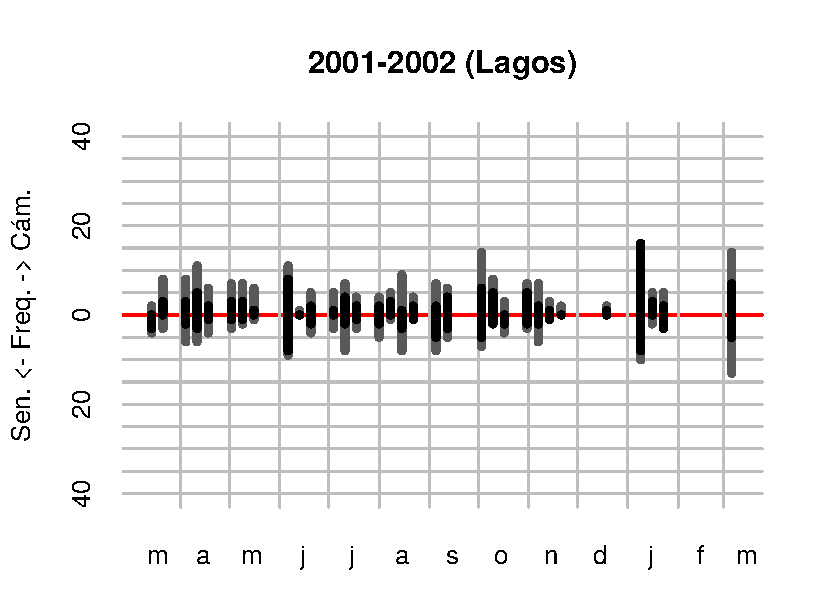
\includegraphics[width=.22\columnwidth]{../graphs/urgenciasHistog2001.pdf} \\
    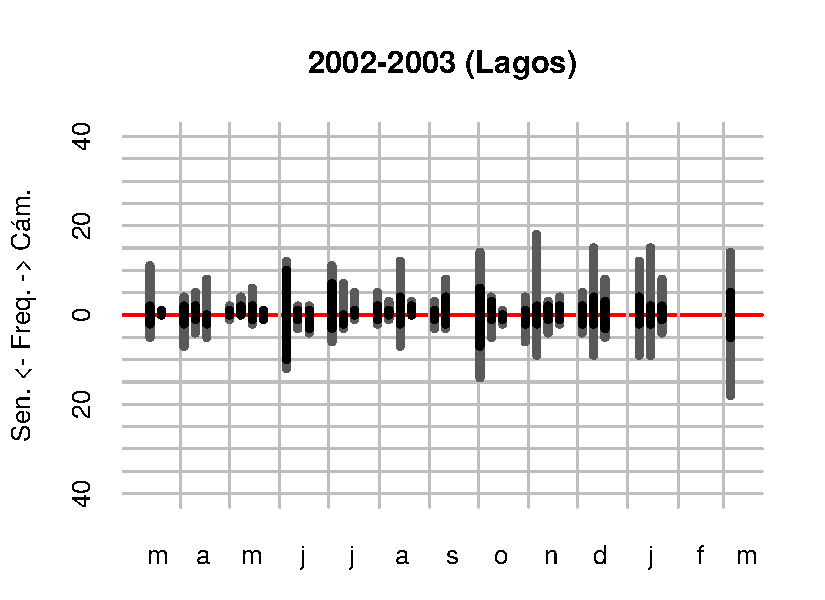
\includegraphics[width=.22\columnwidth]{../graphs/urgenciasHistog2002.pdf} &
    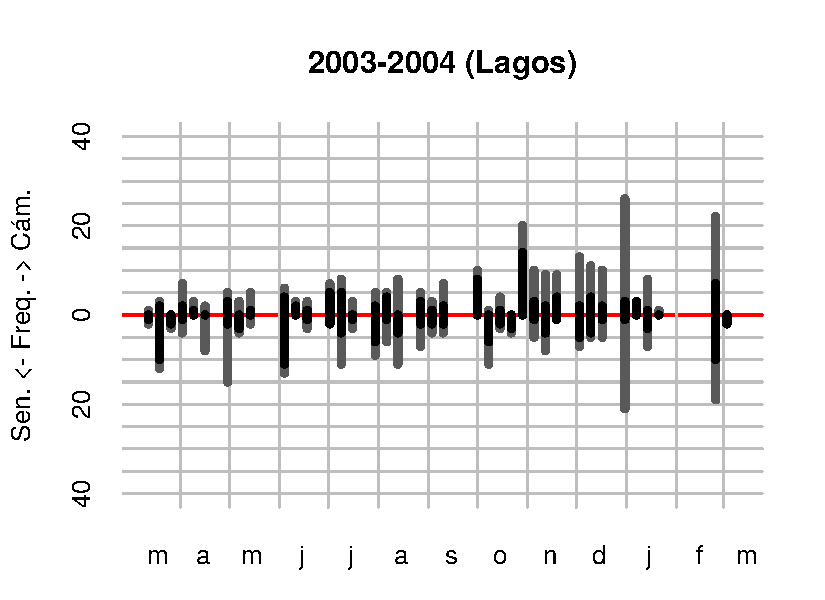
\includegraphics[width=.22\columnwidth]{../graphs/urgenciasHistog2003.pdf} &
    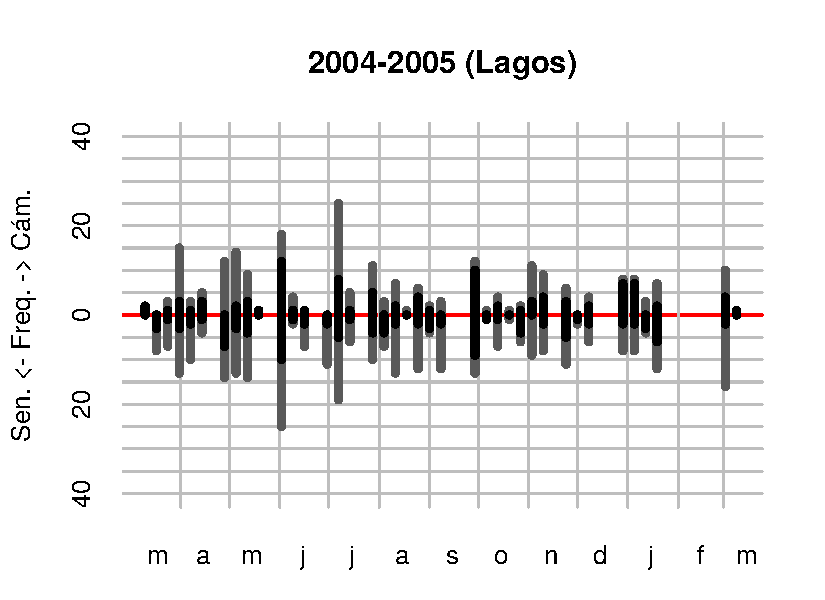
\includegraphics[width=.22\columnwidth]{../graphs/urgenciasHistog2004.pdf} &
    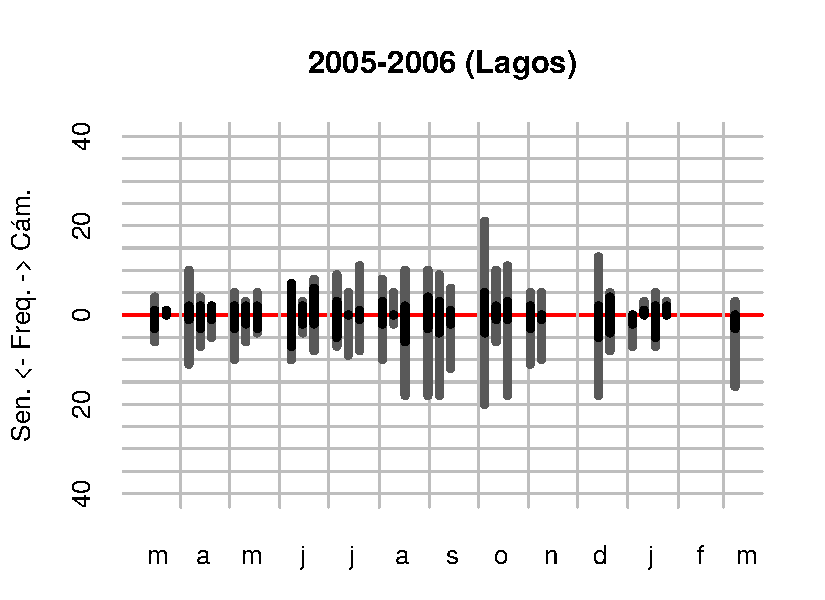
\includegraphics[width=.22\columnwidth]{../graphs/urgenciasHistog2005.pdf} \\
    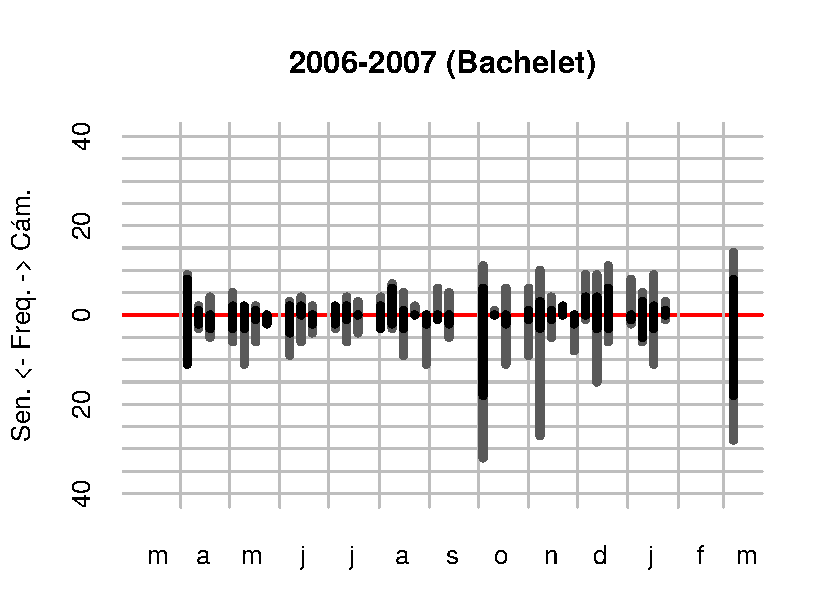
\includegraphics[width=.22\columnwidth]{../graphs/urgenciasHistog2006.pdf} &
    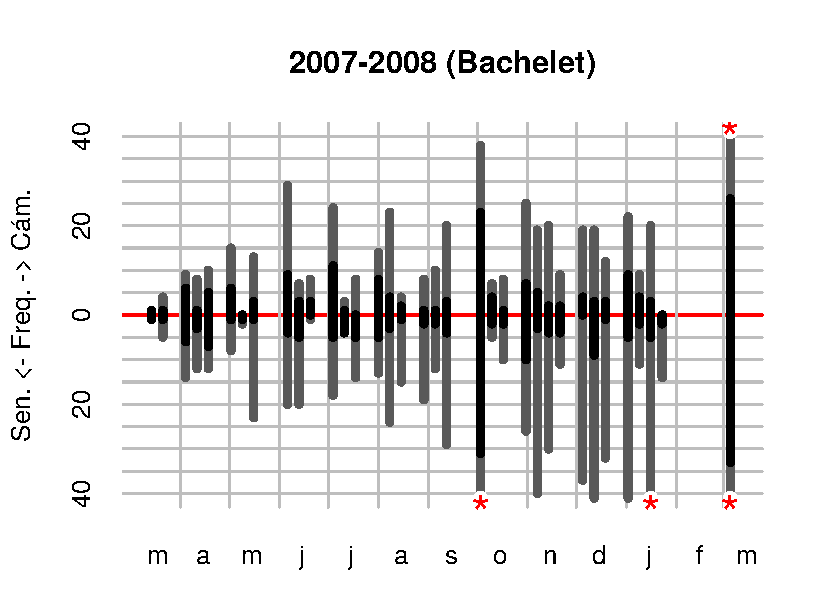
\includegraphics[width=.22\columnwidth]{../graphs/urgenciasHistog2007.pdf} &
    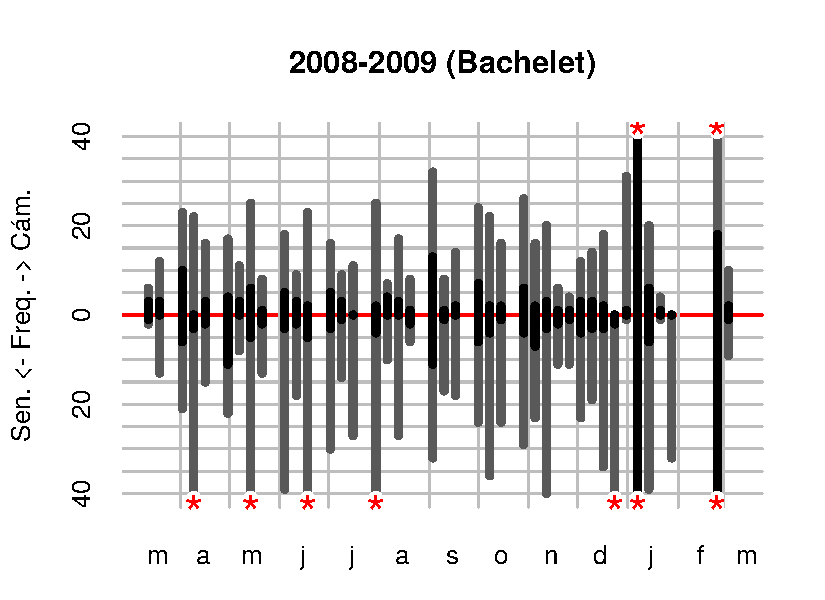
\includegraphics[width=.22\columnwidth]{../graphs/urgenciasHistog2008.pdf} &
    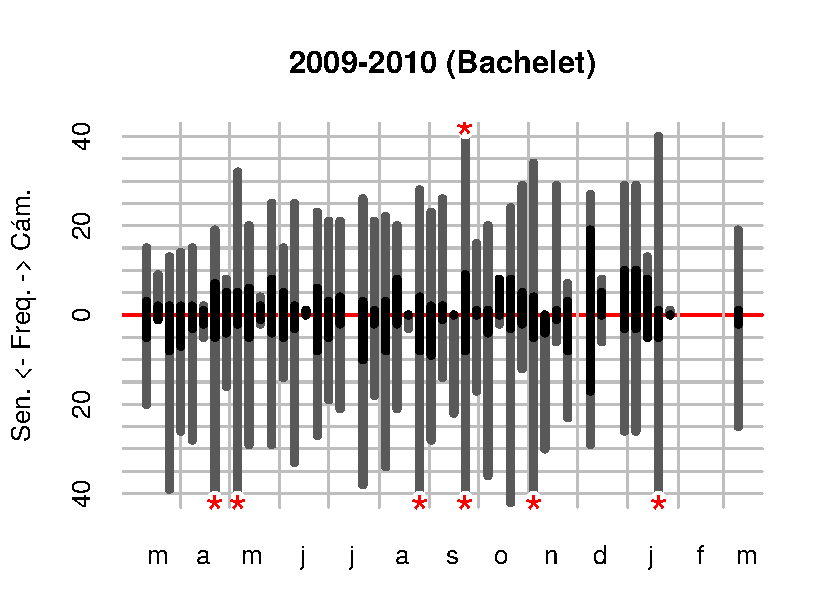
\includegraphics[width=.22\columnwidth]{../graphs/urgenciasHistog2009.pdf} \\
    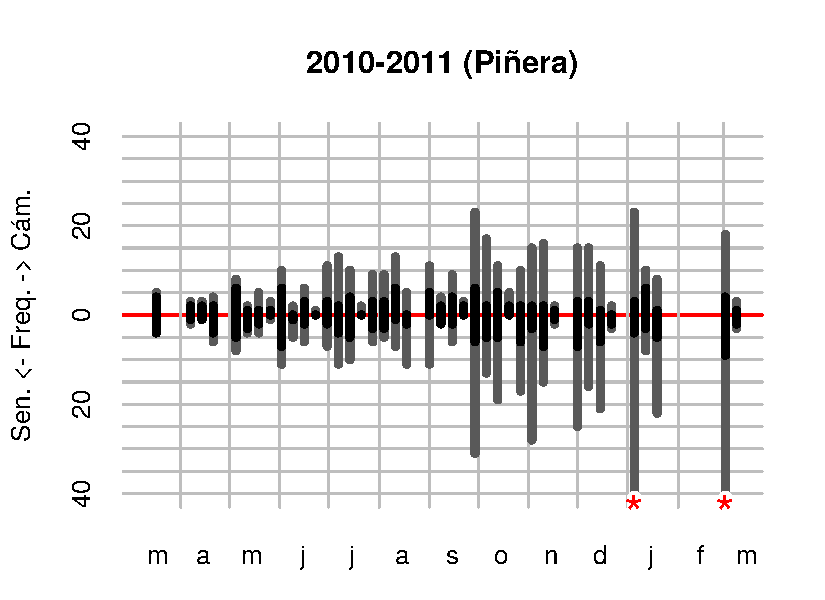
\includegraphics[width=.22\columnwidth]{../graphs/urgenciasHistog2010.pdf} &
    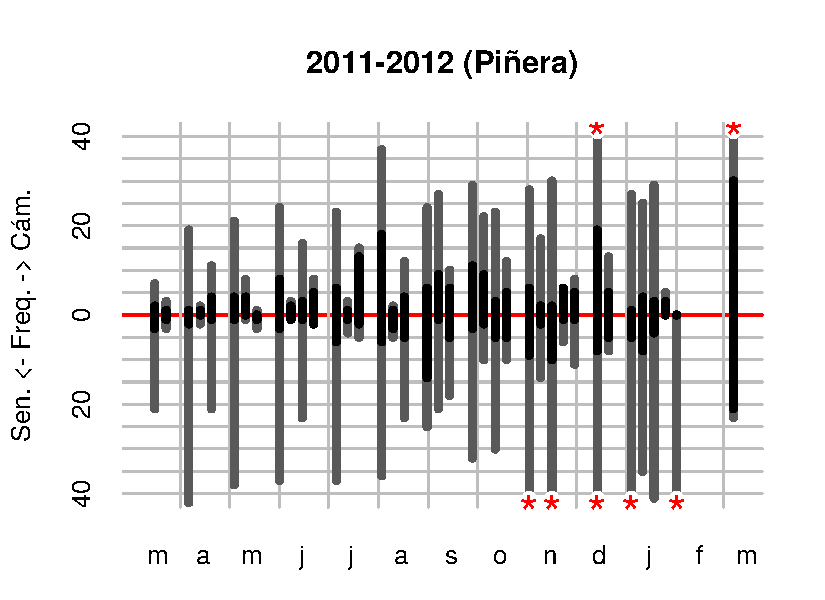
\includegraphics[width=.22\columnwidth]{../graphs/urgenciasHistog2011.pdf} &
    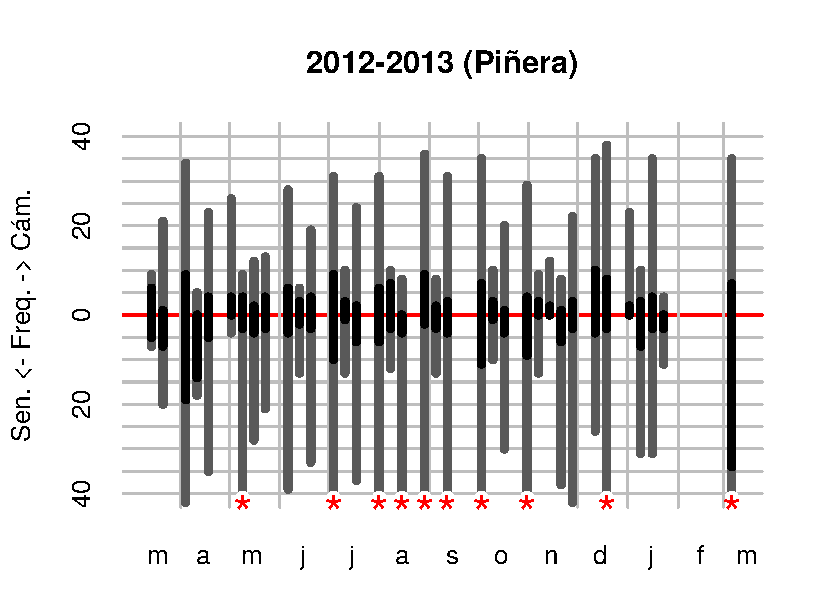
\includegraphics[width=.22\columnwidth]{../graphs/urgenciasHistog2012.pdf} &
    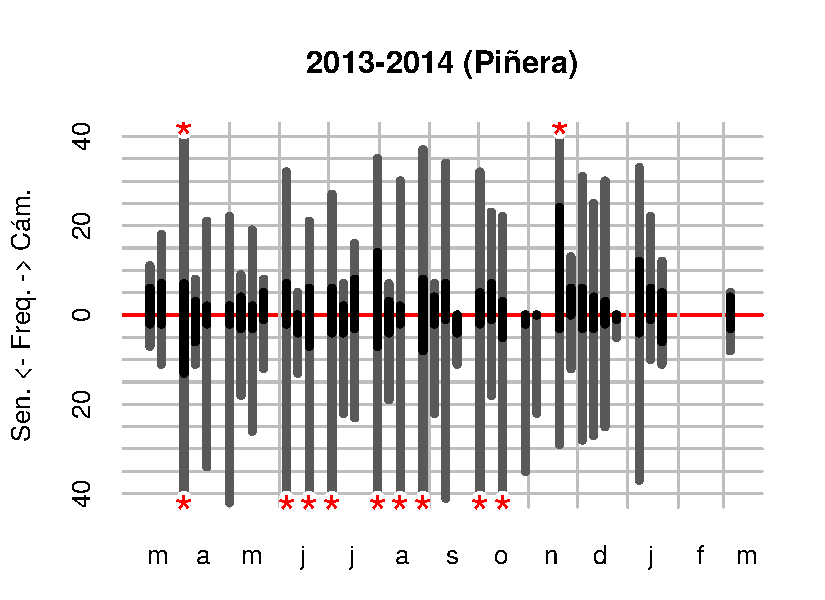
\includegraphics[width=.22\columnwidth]{../graphs/urgenciasHistog2013.pdf} \\
\end{tabular}
  \caption{Weekly urgency messages by legislative year. C\'amara histogram above, Senate below the zero line. Black portion of bars indicates original urgencies, gray portion indicate deadline changes and urgency withdrawals. Asterisk atop column indicates off-the-chart urgency message frequency.}\label{f:depvarHistog}
\end{center}
\end{figure}

% \begin{figure}
% \begin{center}
%     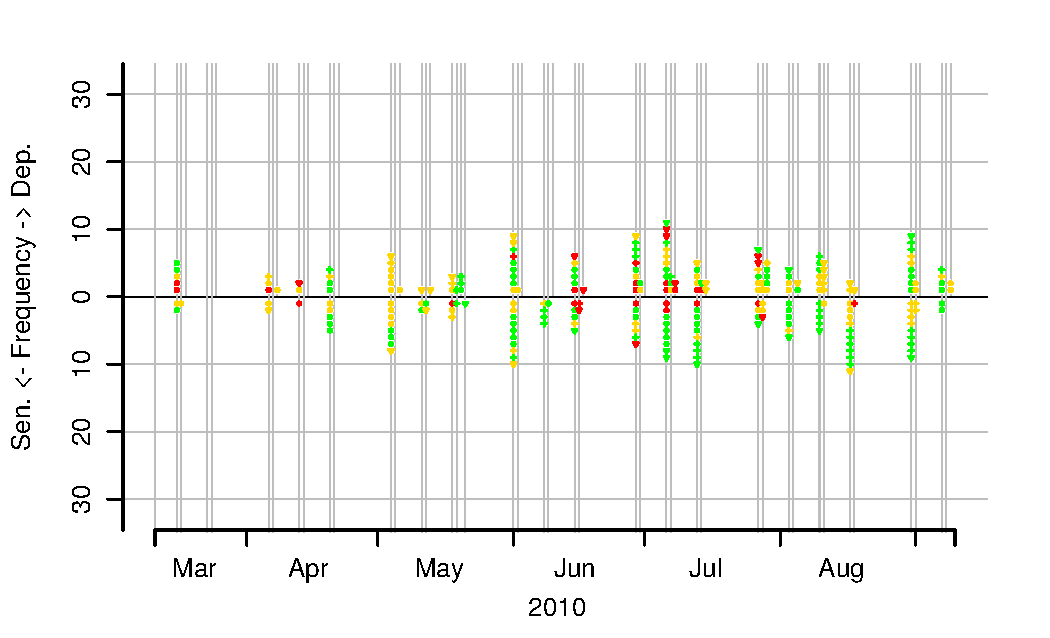
\includegraphics[width=\columnwidth]{../graphs/urgencias2010-1.pdf} \\
%     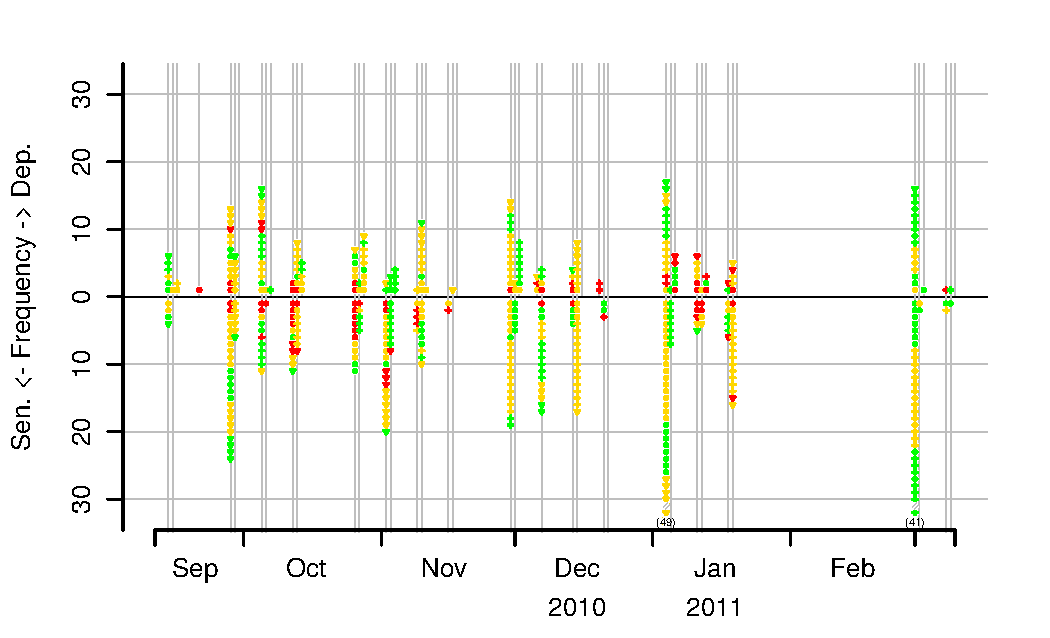
\includegraphics[width=\columnwidth]{../graphs/urgencias2010-2.pdf} 
%   \caption{Urgency messages in legislative year 2010--11. Diputados and Senate data above and below the zero line, respectively. Vertical gray lines indicate that a session took place. One point for each urgency message, a circle for a newly declared urgent bill, a plus sign for an urgent bill with new deadline, a triangle for an urgency withdrawn. Point color indicates the urgency type, red for `act now', yellow for `two week', green for `one month'. Parentheses atop columns indicate off-the-chart urgency message frequency.}\label{f:depvar}
% \end{center}
% \end{figure}

Chains offer a better perspective of the rise in urgency usage. The 170 percent surge between the 2002--06 and 2006--10 Legislatures was, in fact, due to declaring 90 percent more legislation urgent, the rest attributable to substantially longer chains (4.2 links on average, up from 3). The 2010--14 hike is mostly due to longer chains (4.7 links on average), as the chain frequency increase was negligible. Plotting weekly urgency messages in the period, as Figure \ref{f:depvarHistog} does, reveals how original urgency incidence changed little over the years, unlike non-original messages. Each panel in the figure (one of which is zoomed above to provide detail) reports one legislative year as two super-imposed histograms, one for C\'amara and one for Senate messages (both positive scales, red asterisks marking off-the-chart counts). The black portion of columns count original urgency messages, the gray count deadline changes and withdrawals. Note that the evolution of black central segments had some tendency to grow in both chambers from year to year. But that change looks minute compared to how the gray fringes expanded. Urgency-wise, Presidents Bachelet (2006--10) and Pi\~nera (2010--14) had relatively quiet first years in office, using the authority much more often after the second, and especially after the third year. Pi\~nera's more insistent messages to the Senate than the C\'amara, as seen in the red star asymmetry, coincided with a lack of majority in the chamber. 

This temporal dimension in the use of urgencies deserves careful attention in future work. It will be important to disentangle the procedural benefits of the urgency auhtority that we analyze from the actual ``urgency'' aspect of the bill.\footnote{We are grateful to one anonymous referee for pointing this out.}

%Figure \ref{f:depvarHistog} makes the time scarcity very plain. If the urgency authority were consequential, the abundance of messages would pose a genuine scheduling problem for legislators and legislative parties. Is there scheduling time left for member proposals? Not taking the February Summer break into account (when Congress rarely convenes), the C\'amara in the median legislative year had just 4 weeks free of original urgency messages, and none free of urgency messages of either type. **Cite Bond literature in medieval sea trade (Champagne fairs? Weingast? North?)

%% \begin{table}
%% \begin{center}
%% \begin{small}
%% \begin{tabular}{lrrrrrrrr}
%%                          &  \mc{8}{c}{Percent Concertaci\'on sponsors} \\
%% Urgency raised by        &  0\%      &  1--25\%  &  26--50\%  &  51--75\%  &  76--99\%  &  100\%      &  All         &  N \\ \hline
%% Concertaci\'on presidents& \emph{21} & \emph{3}  & \emph{10}  & \emph{15}  & \emph{13}  & \emph{39}   &  \emph{100}  &  228 \\
%% Right president          & \emph{26} & \emph{4}  & \emph{18}  & \emph{12}  & \emph{12}  & \emph{26}   &  \emph{100}  &  121 \\
%% \end{tabular}
%% \caption{Sponsorship of urgent member bills. Entries are relative frequencies of Concertaci\'on sponsors among bills declared urgent by presidents elected by a given list. The first entry reports that 21 percent of bills declared urgent by a Concertaci\'on president had not a single sponsor elected by that list; and so forth.}\label{T:sponsorsOfUrgBills}
%% \end{small}
%% \end{center}
%% \end{table}

%% % ``Para evitar entorpecer el funcionamiento de Congreso, el Ejecutivo procura no tener, al mismo tiempo, más de 10 proyectos con urgencia en cada una de las Cámaras (entrevista Carmona)'' (fn.~25) Carmona citado en berrios gamboa

%% Saturating the agenda with urgent executive bills inevitably plunders scheduling time to consider members' pet projects.\footnote{\citet{berrios.gamboa.fiscChile.2006} quote the executive's legal chief of staff describing a general goal in the Executive branch to have, at most, ten urgent projects in each chamber at once and thus ``prevent blundering congressional work (\emph{evitar entorpecer el funcionamiento de Congreso})'' (fn.~25). It is an optimistic assessment of presidential self-restraint, to say the least. If the urgency authority were consequential, presidents who have taken the chamber's schedule hostage might be a better analogy than self-restraint.} In such circumstances, the urgency authority gives presidents another asset for vote-buying, granting members' projects urgent status in exchange for supporting presidential proposals short of votes in the chamber. Table \ref{T:sponsorsOfUrgBills} has evidence consistent with this possibility: controlling for the percentage of signatures by legislators belonging to Concertaci\'on parties in the proposal reveals that presidents often granted urgent status to opposition bills. Of member bills declared urgent by Concertaci\'on presidents (1998--2010), 21 percent fell in this category, and 26 percent by the right-of-center administration (2010--2014). Another promising area for future research.

  
\section{Model estimates by issue areas and importance}

Controlling bill importance, and even bill's issue areas is no easy task. We offer a preliminary assessment using broad thematic and importance groups. We derived issue areas from the ex-ante categorization that legislative staff assigns upon bill introduction (bill \emph{boletines} include a general category such as Human Rights or Education). We alternatively coded broad issue areas based on the bill's summary (\emph{materia}). The issues we isolated are the following: Agrigulture, fisheries, and the environment; Copper mining and government revenue; Foreign affairs and international treaties; Exports and commerce (parentheses in Figure \ref{F:avgMgSub} indicate whether the classification is with one indicator or the other: bol.\ or mat.) 

We finally relied on a classification of bill importance for most bills initiated by Presidents Bachelet and Piñera. Mayhew’s (1991) outstanding criteria, extended by others (e.g., Cameron 2000; Clinton and Lapinski 2006), is difficult to apply in other contexts because that work relied on the existence of sophisticated media analyses not available in the Latin American setting. We take the variable from Palanza (2020), which considers three levels of significance. This classification is conceptually similar to Mayhew's (1991). 
The three levels identified are: (1) landmark legislation, (2) important legislation, and (3) minor legislation. 

Level 1 – Landmark legislation: This category includes only major pieces of legislation that establish or profoundly reform areas of legislation that have broad effects across the nation. Only extensive and profound reforms to these laws enter this category (narrow reforms are placed in the next category). 

Level 2 – Important legislation: This category includes legislation with varying degrees of importance, yet that ultimately falls short of producing the broad effects of landmark legislation. It includes legislation that reforms aspects of landmark legislation, and legislation that regulates important issues but is constrained in terms of scope. 

Level 3 – Minor legislation: This category includes pieces of legislation that are mostly symbolic or that establish issues that are important only for a very small group of individuals, with minor consequences for the broader population. 

While this classification is available for a sample of the years included in our study (years 2006-2008 and 2010-2013) it covers the first three years of two administrations, one from each of the two coalitions dominating Chilean politics.



\begin{figure}
  \centering
    \caption{Average marginal effect of Coalition Chairs over subsets of bills. Dots report how the probability of an urgent bill changes in response to a unit change in each independent variable, all else at mean values; bars are 95-percent confidence intervals.}\label{F:avgMgSub}
    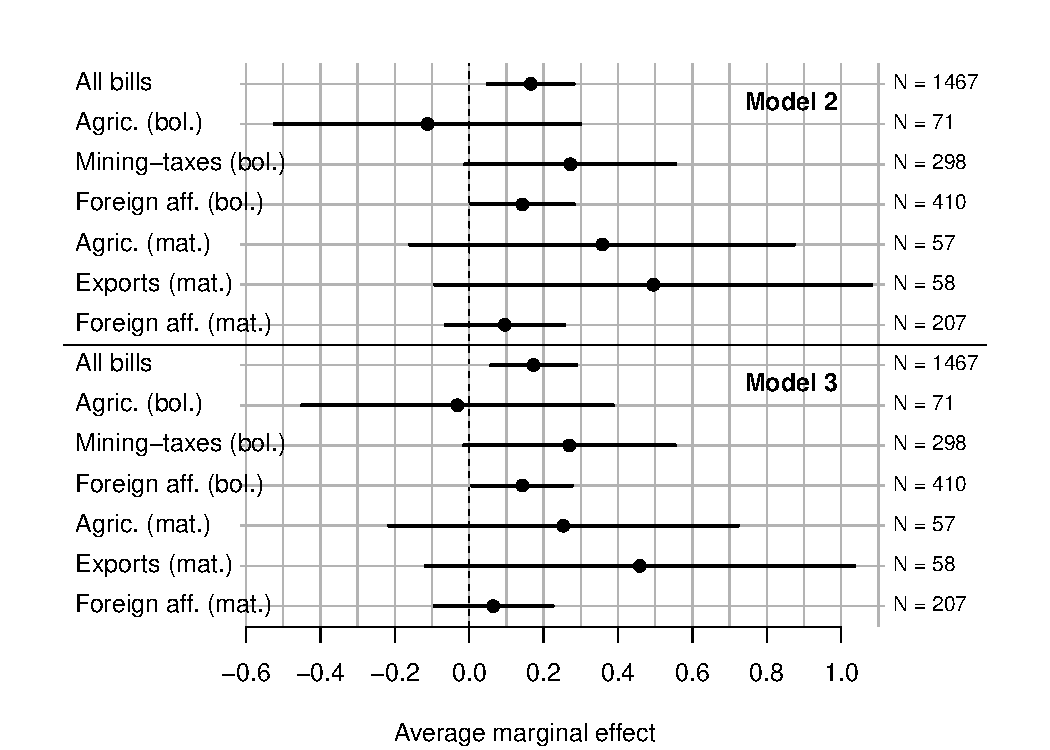
\includegraphics[width=.9\columnwidth]{../graphs/avgMgEffects-subsets.pdf}
\end{figure}

Coefficient estimates mostly fail to achieve statistical significance, likely due to small subsets of bills in categories. But, with the exeption of agriculture (as coded from \emph{boletines}), all point estimates are positive, like those reported in Figure \ref{F:avgMg}. 

Results are also robust to an attempt to control for bill importance. Three-quarters of draft law introduced between March 11, 2006 and March 10, 2014 are categorized as low-, mid-, or high-importance. Estimating the regression on subsets of bills produces results (shown below) in line with those reported in the text. We do not include importance dummies in the reported models because the classification is preliminary and incomplete. 

\begin{table}
\caption{Regressions with rudimentary control for bill importance}
  \begin{singlespacing}
    \begin{footnotesize}
     \begin{verbatim}
Executive bills by importance coding
 Low   Mid    Hi  unclassified    Total
 228   311    49           207      795
(29)  (39)   (6)          (26)    (100)

Signif. codes:  0 ‘***’ 0.001 ‘**’ 0.01 ‘*’ 0.05 ‘.’ 0.1 ‘ ’ 1

Model 3 on low-importance bills only
Coefficients:
                     Estimate Std. Error z value Pr(>|z|)    
(Intercept)           -2.7332     0.8217  -3.326  0.00088 ***
dsameCoal              1.8554     0.8230   2.255  0.02416 *  
dmultiRef              0.9788     0.3531   2.772  0.00557 ** 
drefHda                1.0389     0.3323   3.126  0.00177 ** 
dinSen                -1.1624     0.4202  -2.766  0.00567 ** 
legyrR                -0.1318     0.1510  -0.873  0.38276    
legyrR2               -0.1291     0.1696  -0.761  0.44656    
netApprovR            -0.1710     0.2422  -0.706  0.48013    
as.factor(legis)2010   0.6354     0.3917   1.622  0.10478    

Model 3 on mid-importance bills only
Coefficients:
                     Estimate Std. Error z value Pr(>|z|)    
(Intercept)          -1.89145    0.51059  -3.704 0.000212 ***
dsameCoal             0.89270    0.49111   1.818 0.069109 .  
dmultiRef             1.09446    0.27708   3.950 7.82e-05 ***
drefHda               0.61223    0.27584   2.220 0.026450 *  
dinSen               -0.52883    0.30901  -1.711 0.087018 .  
legyrR                0.07731    0.12743   0.607 0.544071    
legyrR2              -0.14392    0.12936  -1.113 0.265889    
netApprovR           -0.21414    0.17932  -1.194 0.232407    
as.factor(legis)2010  0.97796    0.27170   3.599 0.000319 ***

Model 3 on mid- and high-importance bills only
Coefficients:
                     Estimate Std. Error z value Pr(>|z|)    
(Intercept)           -1.9858     0.4504  -4.409 1.04e-05 ***
dsameCoal              0.7963     0.4308   1.848  0.06454 .  
dmultiRef              1.1485     0.2666   4.308 1.65e-05 ***
drefHda                0.7332     0.2588   2.833  0.00462 ** 
dinSen                -0.4823     0.2983  -1.617  0.10590    
legyrR                 0.1488     0.1194   1.245  0.21301    
legyrR2               -0.1648     0.1209  -1.363  0.17281    
netApprovR            -0.1761     0.1681  -1.048  0.29478    
as.factor(legis)2010   1.0540     0.2602   4.050 5.11e-05 ***
    \end{verbatim}
   \end{footnotesize}
  \end{singlespacing}
\end{table}

\section{Model 2 controlling for the electoral cycle}

Figure \ref{f:depvarHistog} in section \ref{s:temp-dim} of this appendix offers no evidence of an electoral cycle in original urgencies. The gray columns, reporting non-original urgency messages, clearly increased in frequency in the second half of the Bachelet and Piñera administrations (but not before 2006). But the relevant datum for our analysis is reported by the black portion of the columns. As defined in section \ref{s:descriptives-dummies}, the dependent variable equals 1 for bills with at least one supreme urgency in the lower house. The dichotomous nature of the variable makes this equivalent to \emph{original} supreme urgency messages, as subsequent, non-original supreme urgency messages do not increase the value beyond 1. No temporal pattern is discernible in original urgency messages.

\begin{table}
  \begin{footnotesize}
\caption{Model 2 with electoral cycle control (\emph{ptermR})}\label{t:m2elect}
\centering
\begin{verbatim}
Call:
glm(formula = dv ~ dsameCoal + dmultiRef + drefHda + dmajSen + 
    dinSen + legyrR + legyrR2 + ptermR + ptermR2 + dreform2010 + 
    netApprovR, family = binomial(link = logit), data = tmpdat, 
    subset = dmocion == 0)

Deviance Residuals: 
    Min       1Q   Median       3Q      Max  
-1.8788  -0.9139  -0.6284   1.0844   2.3639  

Coefficients:
            Estimate Std. Error z value Pr(>|z|)    
(Intercept) -1.40487    0.35329  -3.976 6.99e-05 ***
dsameCoal    0.82930    0.29636   2.798 0.005137 ** 
dmultiRef    0.77807    0.13211   5.890 3.87e-09 ***
drefHda      0.94992    0.12404   7.658 1.89e-14 ***
dmajSen     -0.43955    0.20721  -2.121 0.033901 *  
dinSen      -0.72349    0.17274  -4.188 2.81e-05 ***
legyrR       0.06244    0.06235   1.001 0.316628    
legyrR2     -0.23623    0.06521  -3.623 0.000292 ***
ptermR       0.13662    0.06583   2.075 0.037967 *  
ptermR2     -0.11736    0.07301  -1.608 0.107943    
dreform2010  0.35792    0.24294   1.473 0.140678    
netApprovR  -0.03405    0.08051  -0.423 0.672311    
---
Signif. codes:  0 ‘***’ 0.001 ‘**’ 0.01 ‘*’ 0.05 ‘.’ 0.1 ‘ ’ 1

(Dispersion parameter for binomial family taken to be 1)

    Null deviance: 1930.4  on 1466  degrees of freedom
Residual deviance: 1718.4  on 1455  degrees of freedom
AIC: 1742.4

Number of Fisher Scoring iterations: 4
\end{verbatim}
\end{footnotesize}
\end{table}

We nonetheless estimated our regression model controlling for the 4-year election cycle, reported in Table \ref{t:m2elect}. Variable \emph{ptermR}, and its square to capture a non-linearity, are defined analogously as \emph{Year Remaining} (referred to as \emph{legyrR} in this table)---it is the percentage of the presidential term remaining at bill initiation (normalized for comparability with the reported model). The linear coefficient is statistically significant but indicates that, other things constant, there is a drop as the next election nears. The important point here is that other coefficients are virtually unchanged, so we prefer to report the simpler model omitting this control. 

\section{Comparative statics}

Pay attention to consideration regimes in Figure \ref{F:predictions}. Magenta status quos trigger the fast-track, white ones do not. (The gray lack a consideration regime because the committee does not report the bill). Fast-track conditions behind magenta rectangles generalize thus:  

\begin{description}
\item[\textsc{Condition 1} (necessary)] relative to $F$, $C$ and $P$ are on the same side; 
\item[\textsc{Condition 2} (sufficient)]  $q \notin [C,F]$ \& \textsc{condition 1};
\item[\textsc{Condition 3} (necessary and sufficient)] $q \notin [min(C_{P_F},C),F]$ \& \textsc{condition 1}.
%\item[\textsc{Condition 2} (sufficient)]  $q \notin ([C,F]\text{ or }[F,C])$ \& \textsc{condition 1};
%\item[\textsc{Condition 3} (necessary and sufficient)] $q \notin ([min(C_{P_F},C),F]\text{ or }[F,max(C_{P_F},C)])$ \& \textsc{condition 1}.
\end{description}


%% %%%%%%%%%%%%%%%%%%%%%%
%% % APPENDIX ENDS HERE %
%% %%%%%%%%%%%%%%%%%%%%%%



\end{document}
